%
% Modified by Megan Patnott
% Last Change: Jan 18, 2013
%
%%%%%%%%%%%%%%%%%%%%%%%%%%%%%%%%%%%%%%%%%%%%%%%%%%%%%%%%%%%%%%%%%%%%%%%%
%
% Modified by Bryce Frentz
% Last Change: 2018
%
%%%%%%%%%%%%%%%%%%%%%%%%%%%%%%%%%%%%%%%%%%%%%%%%%%%%%%%%%%%%%%%%%%%%%%%%
%
% Sample Notre Dame Thesis/Dissertation
% Using Donald Peterson's ndthesis classfile
%
% Written by Jeff Squyres and Don Peterson
%
% Provided by the Information Technology Committee of
%   the Graduate Student Union
%   http://www.gsu.nd.edu/
%
% Nothing in this document is serious except the format.  :-)
%
% If you have any suggestions, comments, questions, please send e-mail
% to: ndthesis@gsu.nd.edu
%
%%%%%%%%%%%%%%%%%%%%%%%%%%%%%%%%%%%%%%%%%%%%%%%%%%%%%%%%%%%%%%%%%%%%%%%%

%
% Chapter 2
%

\chapter{Experimental setup and procedures}
\label{chap: experiment}

\section{Introduction}

This chapter is included to highlight some techniques and equipment commonly used in low-energy nuclear physics, with an emphasis on those used in this work. The discussion will be presented from the lens of the general to the specific, introducing general concepts for beam production and transport, acceleration systems, and radiation detection. Following the discussion of the scientific principles, I will detail the specifics of the equipment employed in this collective work. To that end, I will also highlight differences between the facilities and techniques employed when compared to common equipment for nuclear physics experiments


\section{Experimental Equipment}
\label{sec: equipment}



\subsection{Accelerators}
\label{sec: accelerators}

First and foremost, low-energy nuclear physics (generally understood to be the regime in which incident kinetic energies for reactions are below 1 GeV, often even as low as sub-MeV) requires particle acceleration systems in order to bring beams and targets together. The most common techniques for accelerating ions are 1) to use strong electrostatic fields for a straight-line acceleration, such as in the Van de Graaff accelerator, or 2)  by using a combination of electric and magnetic fields to accelerate the particles in cyclotron motion, aptly named a cyclotron. Van de Graaff accelerators are the most prominent of all accelerators, though, and are the type used in this work. 

The basic idea of a Van de Graaff accelerator is shown in Fig. \ref{fig: vdg principles}. The governing principle is that a beam of ions produced in an ion source (Section \ref{sec: ion sources}) are manipulated by additional electromagnetic elements (Section \ref{sec: beamline}) into an area of high electric potential. This high voltage is produced and maintained by continuously transporting positive charge from ground to a Faraday cage with a field free interior (referred to as the terminal, with voltage $V_{T}$). The positively charged ions, being in close proximity to the positively charged terminal feel a repulsive force, accelerating the ions out of the terminal and through the machine. Upon exiting the accelerator, the ions have energy

\begin{equation}
E_{ion} = qV_{T} = \dfrac{1}{2} m_{ion} v_{ion}^{2}
\label{eqn: accelerator}
\end{equation}

\noindent where $V_{T}$ again is the terminal voltage and $q$ is the charge state of the ion going through the accelerator, $m_{ion}$ is the mass of the ion, and $v_{ion}$ is the ion's velocity. When the terminal voltage is in MV, the beam energy is then provided in MeV. Specifically for the 5U accelerator, though, Equation \ref{eqn: accelerator} must be modified with an additional term. Inside the ion source, there is an electrostatic extractor, which transports the beam of ions out of the terminal and into the acceleration tube. With this correction, the beam energy for the 5U is given as

\begin{equation}
E_{ion} = q(V_{extractor} + V_{T}).
\label{eqn: beam energy}
\end{equation}

\begin{figure}
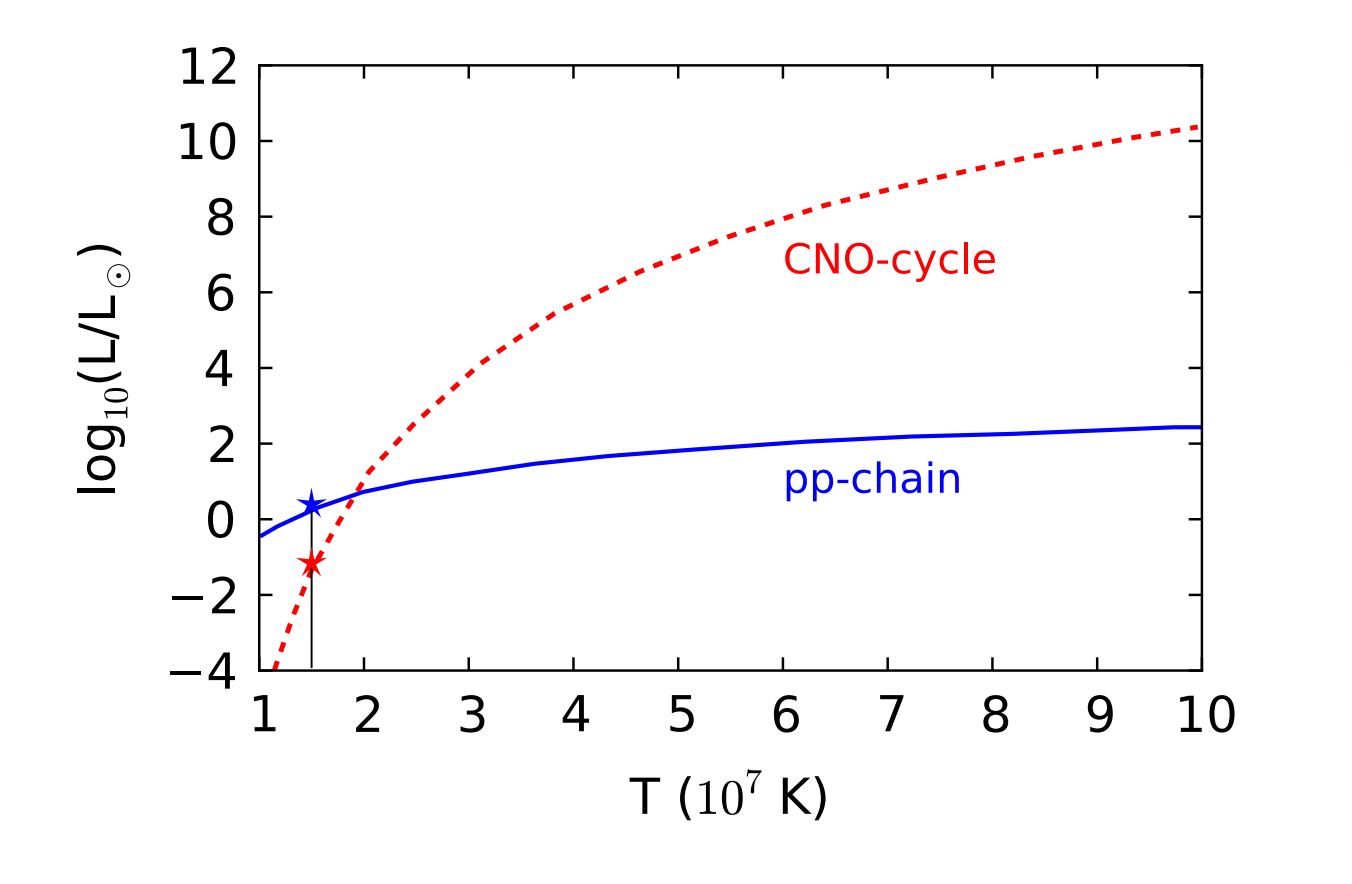
\includegraphics[width=\linewidth]{figures/energyProduction.png}
\label{fig: vdg principles}
\caption{A diagram of a Van de Graaff accelerator \cite{RolfsBook}. The charge transportation in this figure is shown with a belt, like the JN accelerator model at CASPAR, while the 5U accelerator at the NSL uses a Pelletron chain. }
\end{figure}

The charge is delivered to the terminal via a mechanical delivery system. The 5U Sta. Ana accelerator at the NSL uses four Pelletron chains cite{Herb1974}, each with its own power supply, while the JN Van de Graaff accelerator at CASPAR utilizes a rotating belt. In either case, the entire charging system is contained inside of a pressurized tank of insulating gas, SF$_{6}$ for the 5U and CO$_2$ for the JN, reducing the chance of a terminal discharge to ground from dielectric breakdown. This is not the only element to ensure the operational stability of the machine. The charging systems supply charge continuously to the terminal. However, charge is always being removed from the terminal via three primary pathways: 1) the beam of ions passing through the accelerator, 2) the resistive column, and 3) the corona system. In order to maintain stability, the currents that pass through these systems must always be in balance according to Kirchoff's Rule,

\begin{equation}
I_{chains} = I_{beam} + I_{column} + I_{corona}.
\end{equation}

\noindent The column is actually a series of equipotential hoops connected by equal resistors. Each conducting hoop provides a small step down in voltage from the terminal, ensuring that the beam of ions feel a smooth potential gradient throughout their acceleration. These can be seen in Fig. \ref{fig: column}, showing an interior view of Sta. Ana accelerator tank. 


\begin{figure}
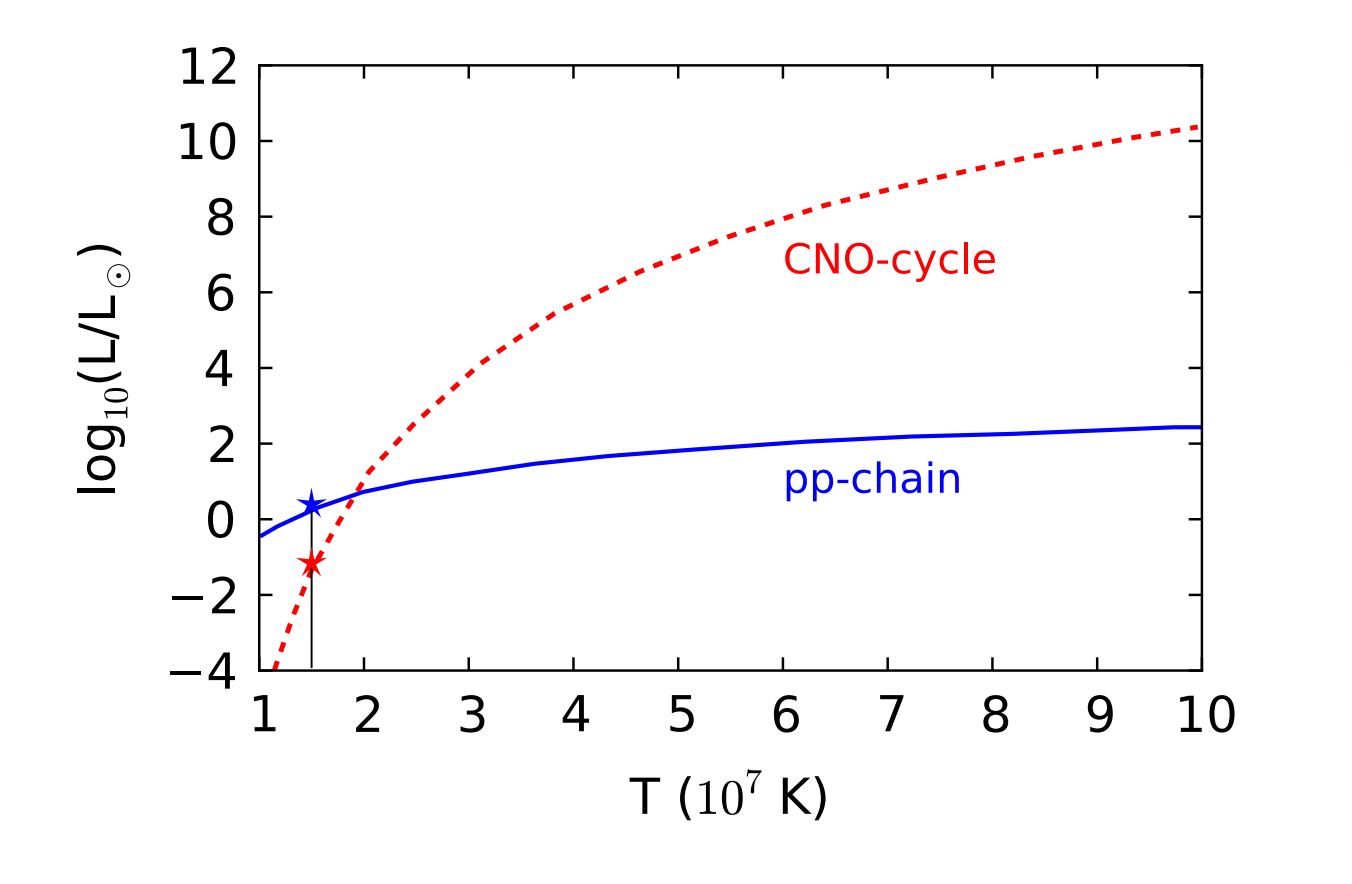
\includegraphics[width=\linewidth]{figures/energyProduction.png}
\label{fig: column}
\caption{View inside the Sta. Ana accelerator tank, showing the equipotential hoops as part of the column.}
\end{figure}


The corona system is the real workhorse maintaining the stability of the accelerator's charging systems. As small irregularities can be present between different links in the Pelletron chains or the belt itself, the corona system is responsible for precise second-by-second compensation. The mechanical part of the system consists of an arm with sharp metal points on the end which can be moved towards and away from the terminal to draw away current. On the back end, however, it also is controlled by a voltage feedback system to adjust the current draw, keeping the terminal at a constant voltage. The feedback for the system is provided either by an external reference through a generating voltmeter or from the beam itself as it passes through an analyzing dipole magnet at the exit of the accelerator. As the beam passes through the magnet it will pass through a set of slits. If $V_{T}$ changes slightly, the energy of the beam will subsequently change, impacting the balance of the beam on the exit slits. This change in current will be fed back to the corona system, which in turn will compensate by changing the charge delivered to the terminal in order to maintain the slit balance. With this, $V_{T}$ can be kept incredibly steady, within roughly 1 kV for every MV on the terminal. This is the biggest advantage of a Van de Graaff accelerator over a cyclotron. Intrinsically, this acceleration system makes nuclear experiments possible through monoenergetic beams. 


\subsection{Ion sources}
\label{sec: ion sources}

A key item for the successful operation of any accelerator is the ion source, which produces the beams of charged particles used in experiments. Generating such beams is not a trivial task and, as such, many methods have been developed for achieving this. The two types relevant to this work, however, are the Electron-Cyclotron Resonance (ECR) ion source, used in the Sta. Ana accelerator at the NSL, and the radio frequency (RF) ion source, utilized in the JN accelerator at CASPAR.  Both systems are housed within their respective accelerator terminals, which acts as a Faraday cage and shields the internal components from external fields. Additionally, both systems operate on the same basic principle, namely that a given gas is ionized through the use of electron collisions in the source, but the mode of electron excitation is different. 

For the specifics of the ECR system, the 5U employs a Pantechnik Nanogen 14.5 GHz ECR source. This utilizes the cyclotron resonance of electrons (as the name obviously implies) to produce and maintain a plasma.


\begin{figure}
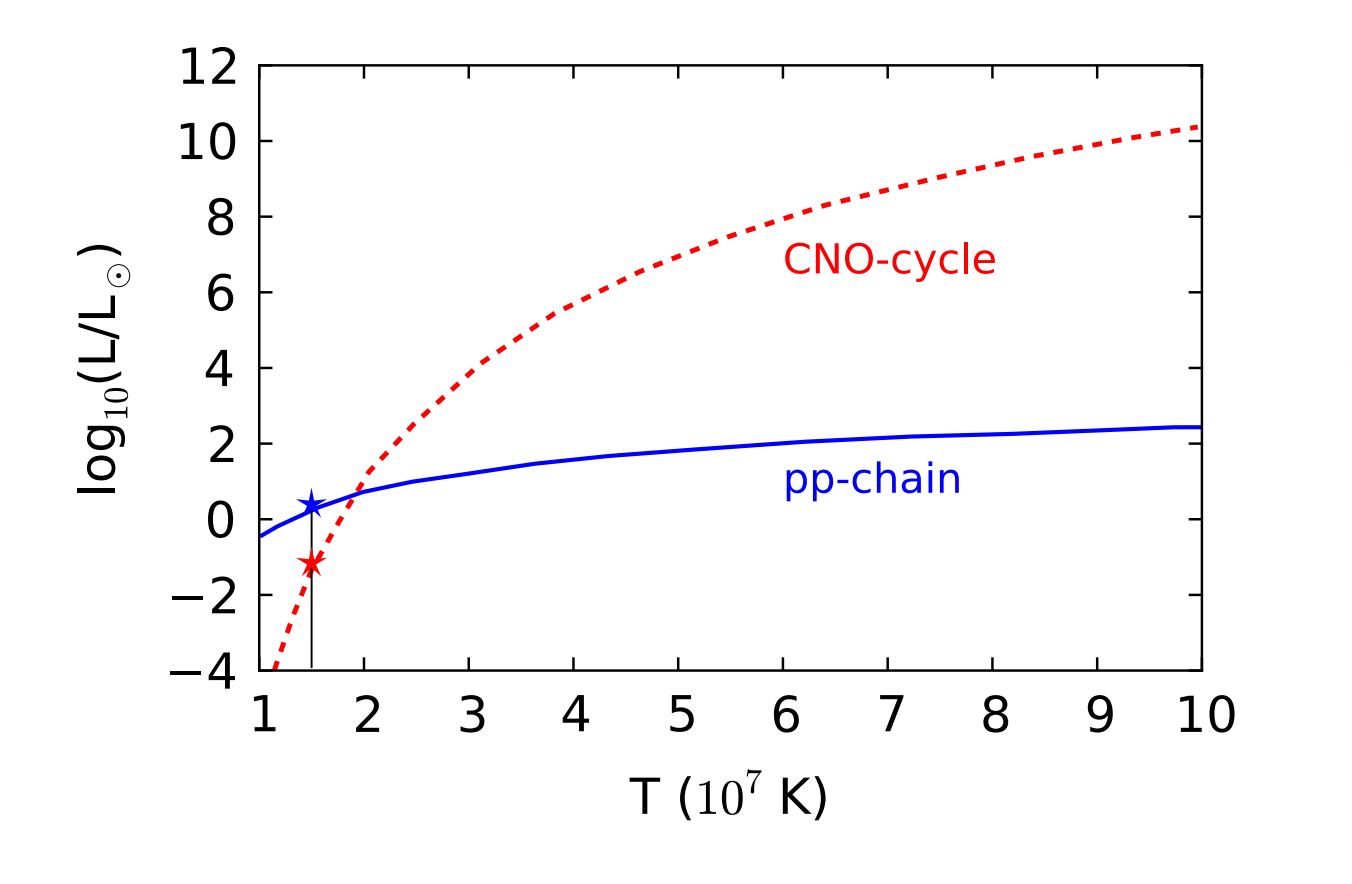
\includegraphics[width=\linewidth]{figures/energyProduction.png}
\label{fig: ecris}
\caption{Depiction of the interior of an ECR ion source with magnetic components labeled cite{Melin1997}. This example shows a source operating from left to right, with the gas and RF generator inputs depicted as well as the exit for the ions. As discussed in the text, the combination of magnets confines the plasma in the center as it is pushed from left to right and out of the source.}
\end{figure}


During operation, neutral gas (which includes the element to be accelerated as a component) is injected into a cavity surrounded by magnets. These magnets provide a superposition of axial and multipole fields in order to achieve a minimum at the center of the cavity increasing radially outwards with the goal of confining and stabilizing the generated ions. A cartoon depiction of such a system is presented in Fig. \ref{fig: ecris}. In order to generate the ions from neutral gas, a current is supplied to the chamber by a negative bias probe providing a constant supply of charge. From this, then, electrons are stripped and continually accelerated in cyclotron motion following the familiar cyclotron frequency relation:

\begin{equation}
\omega_{ecr} = \dfrac{e | B |_{ECR}}{m_{e}} = \omega_{rf}
\label{eqn: ecr}
\end{equation}

\noindent where $\omega_{ecr}$ is the frequency for the cyclotron resonance of electrons in a given magnetic field $B_{ECR}$, $e$ and $m_{e}$ are the charge and mass of the electron, respectively, and $\omega_{rf}$ is the frequency supplied by a radio radio-frequency (RF) power supply. This last term is included to highlight that during operation this is supplied externally and controlled in the use of the source in order to produce the plasma. After ionization, the magnetic configuration confines the plasma radially, while the axial magnetic field (provided by the extractor) pushes it through the cavity towards the exit of the source. Upon exiting the chamber and the Faraday cage of the terminal, the positive ions are next to a the positively charged terminal at high voltage, thus accelerating the ions. 

An ECR ion source has many advantages of over other common ion source designs. The primary advantage lies in its ability to deliver high-intensity beams (as much as hundreds of $\mu A$). For use in nuclear astrophysics experiments, such as the ones performed in this work, low cross sections are a problem to overcome, which is mitigated through this higher production. Additionally, due to the relatively simple restrictions on the inputs, these sources can provide a wide array of species, as they can produce beams of nearly anything that can be made into a gas, and exhibit long term stability, reliability, and longevity cite{Melin1997}.  On the other hand, however, ECR ion sources also have some disadvantages compared to other common sources. One main drawback is that the ions are produced through the production of a plasma, meaning they are not directly controlled by any operational parameter cite{Melin1997}. This leads to complicated tuning and sensitive operation, experimentally. Additionally, such sources are only capable of generating positive beams and can therefore only be utilized in single stage accelerators. Finally, due to the size of these ion sources and their necessary components, they are often impractical. In order to employ one in the Sta. Ana accelerator, the accelerator design had to be vertical. If the accelerator had been horizontal (like the other accelerators at the NSL) the torque generated by the ECR ion source would have shattered the acceleration column. Vertically, however, the source is stable inside the accelerator. Unfortunately, the choice to build and use the accelerator vertically is not one that every lab can make. 

The radio frequency (RF) ion source utilized at CASPAR operates on a very similar principle to the ECR ion source inside the Sta. Ana accelerator. A depiction of the RF ion source's components is given in Fig. \ref{fig: rfis}. In this case, the source chamber is a glass tube filled with a monoatomic gas, at CASPAR the only options are $\ce{^{1}H}$ and $\ce{^{4}He}$.  Electromagnetic coils are placed on both sides of this tube and generate RF waves in the tube, between the rings. In response to these waves, the electrons oscillate through and collide with the source gas, ionizing it. At the rear of the glass tube, an electrode supplies a constant, positive voltage (with respect to the terminal), forcing any ionized atoms towards the exit of the source. Upon leaving the source, as with the ECR ion source, the ions are accelerated because of their repulsion to the positively charged terminal. 

\begin{figure}
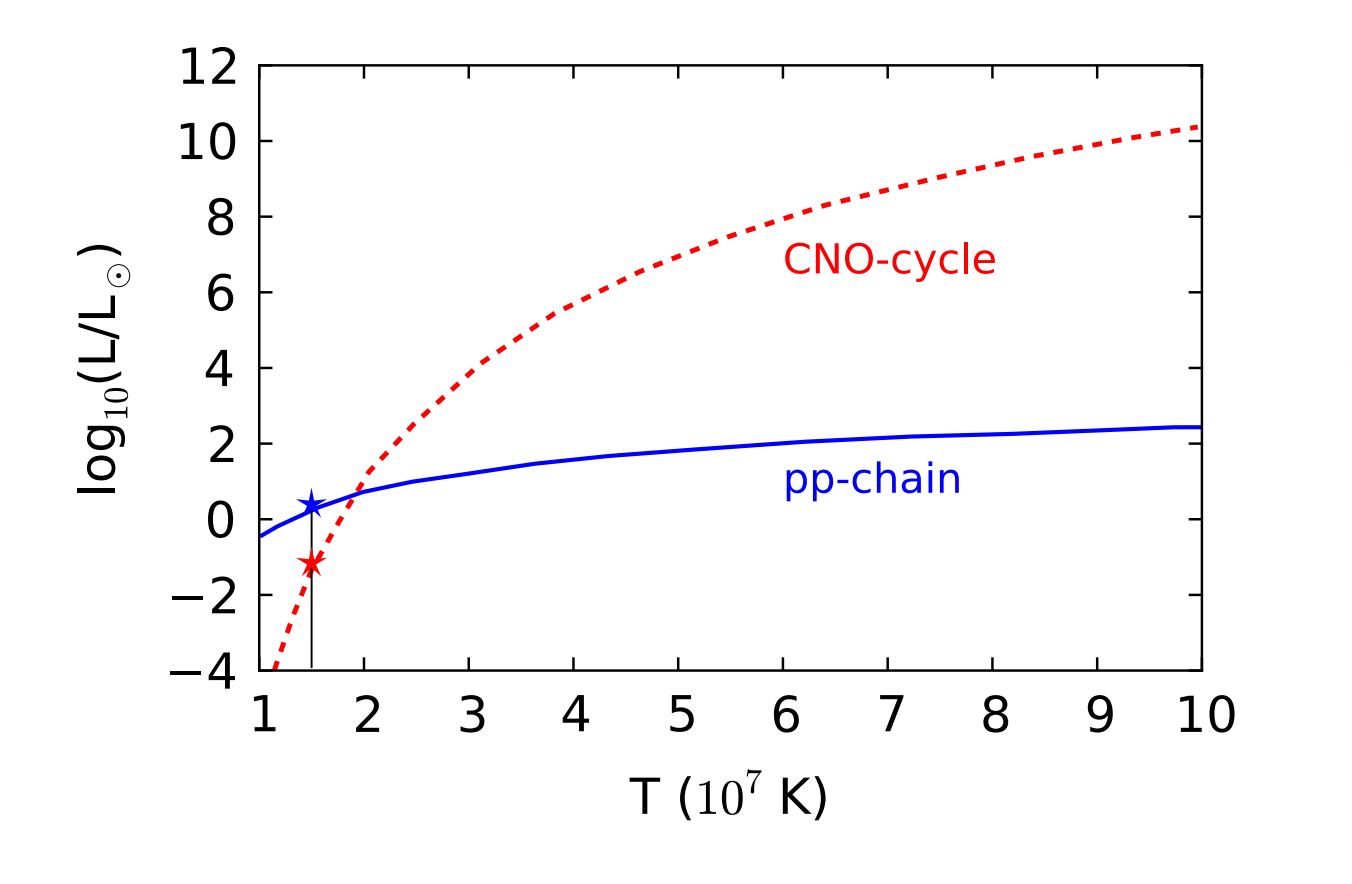
\includegraphics[width=\linewidth]{figures/energyProduction.png}
\label{fig: rfis}
\caption{Depiction of the interior of a RF ion source with magnetic components labeled cite{Li2015}. The coils on either side provide the field to ionize the gas, whereas the probe on top provides the field necessary to extract the ions from the chamber.}
\end{figure}

The RF ion source at CASPAR was also recently refurbished before installation, leaving it capable of beam production at even higher intensities than the ECR ion source inside the Sta. Ana accelerator. It can produce beams up to 150 $\mu A$, enabling similar high-intensity experiments. Another similarity to the ECR ion source is that it provides excellent operational stability and reliability. It does, however have significant drawbacks as well. The first and foremost of these is the degredation of the ion source canal. Operating the source causes a buildup on the exit canal of the source tube (higher intensity operation accelerates this process), necessitating significant maintenance. Additionally, the glass tube housing the plasma is quite sensitive. If power is supplied to the source when gas is not present, significant damage to the tube can occur. This is only mitigated with vigilant operation. The other major drawback is that the source is only capable of providing beams of two species (typically hydrogen and helium). In order to change the delivered species, a full tank opening and source alignment is required. 

Altogether, though, these sources are ideal for this work. They provide the necessary ion beams at high intensity, enabling the experiments. 




\subsection{Beam transport}
\label{sec: beamline}


Upon exiting the accelerator, the beam envelope contains a distribution of different masses, charges, and energies because the ion sources are indiscriminate in their production methods. For example, an ion source might produce some ionized diatomic gas, instead of monoatomic, like producing $\ce{^{1}H}+\ce{^{1}H}$ due to insufficient breakup of the source gas. However, all particles created in the same ionization state will have the same energy, dictated by Equation \ref{eqn: beam energy}. In order to filter such contaminants out of the beam, analyzing magnets are employed. These are typically 90$^{\deg}$ dipole magnets, also utilizing the cyclotron motion of ions in a magnetic field in order to select a given type of particle at a specific energy. These magnets are typically located at the exit of accelerators, and, due to their fixed size, have a fixed radius, $R_{am}$, through which a beam can pass. Therefore, for a given particle of mass $m$, energy $E$, and charge state $q$, the magnetic field, $B_{am}$, inside the analyzing magnet can be tuned to allow through only a specific particle/energy combination by

\begin{equation}
B_{am} = \dfrac{\sqrt{2 m E}}{q R_{am}} = \dfrac{\sqrt{2m}}{q R_{am}} \sqrt{E} = k \sqrt{E}
\label{eqn: analyzingMagnet}
\end{equation}

\noindent, where $k$ is a constant for a unique combination of particle and charge state. This separates the in-beam contaminants from the ions of experimental interest.  

In order to deliver the beam of ions to the target chamber and experimental hall, a series of steering and focusing elements are placed along the beam pipes. As the beam is self-repulsive due to it all being the same charge, these are necessary to contain the beam and keep its intensity at acceptable levels for experimental purposes. They also allow adjustment of the beam's position in order to deliver it to a specific experimental setup and allowing for simple transitions between different target locations. 

Vacuum systems are important components of the beam production and experimental operation. All experimental components, like the ion source chamber, acceleration tubes, target chamber, and connecting beam pipes need to be free of residual gas. If not, the beam quality would suffer dramatically, collisions of the beam with the remaining atmosphere would cause significant intensity and energy losses, preventing transport and, ultimately, the measurement. In order to maintain an experimental vacuum level (typically $\sim 10^{-7}$ Torr), a series of metal pipes run from the ion source to the target chamber. These are connected by air-tight gaskets and have isolating valves employed with high-vacuum pumps (cryogenic or turbomolecular) along the line. These enable easier maintenance or changing of experimental conditions without destroying the vacuum created through the entire beam line. Without high-vacuum, there would be additional adverse effects on the target quality. Contaminants, typically hydrocarbons, present in residual gas can accumulate on the surface of the target due to the beam heating the surface. This is unwanted, as it not only provides an additional layer of energy loss for the beam before interacting with the target but also a significant contaminant in experimental results due to carbon's high cross-section.

Besides maintaining clean, high-vacuum near a target, another common method for reducing the carbon build-up on experimental surfaces is to utilize a so called cold trap in front of a target. A cold trap is is a liquid nitrogen cooled copper pipe designed to be nearly the same size and shape as the beam pipe to prevent it from interfering with an experiment. An example of a cold trap like the one used in this work is shown in Fig. \ref{fig: coldtrap}. The cold trap works much like a cryogenic pump. By cooling the copper pipe with liquid nitrogen, the residual hydrocarbons in the beam pipe and target chamber will condense on the surface of the pipe, trapping them before most can reach the target and cause carbon buildup. 


\begin{figure}
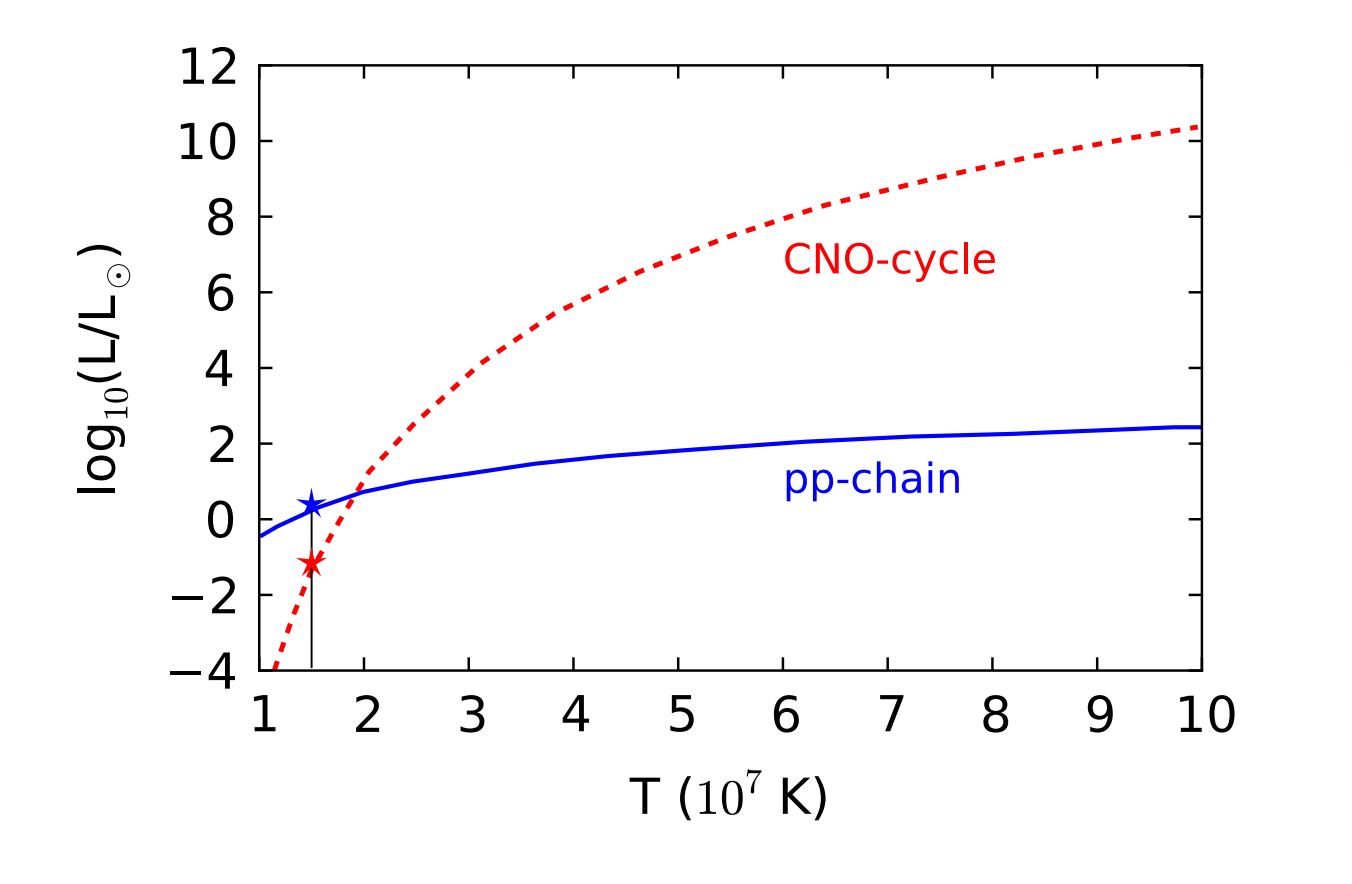
\includegraphics[width=\linewidth]{figures/energyProduction.png}
\label{fig: coldtrap}
\caption{Depiction of a cold trap used in this work. The reservoir on top is filled with liquid nitrogen and connected to the copper pipe inside the target chamber, causing the copper pipe inside to be cooled. At cold temperatures, most of the contaminants present in the beam pipe will condense on the copper pipe instead of building up on the target surface.}
\end{figure}



\subsection{Radiation detection}
\label{sec: detectors}



types

photon interactions with matter

HPGe


\section{The CASPAR facility and cross-section measurements}
\label{sec: cs experiment}



This set of data was taken over the course of five* separate experiments. The first occurred at the University of Notre Dame's Nuclear Science Laboratory (NSL) in January of 2018 and covered the proton energy range of E$_{p}$ = 800 - 1200 keV. The experiment was then continued at the Compact Accelerator System for Performing Nuclear Astrophysics (CASPAR) facility at the Sanford Underground Research Facility located in Lead, South Dakota in three increments: February 2018, May 2018, and August / September 2018. These measurements covered the energy range from E$_{p}$ = 270 - 1200 keV, in order to measure the $^{14}$N$\left( p,\gamma \right) ^{15}$O reaction cross-section to compare the performance of the CASPAR facility to an above-ground laboratory. Finally, in MONTH TIME DATE THING, the final experiment was completed at the NSL, focusing on obtaining the lifetime of the 6793 keV state in $^{15}$O.

Reiterate why we went underground and its advantages
Background comparison

Describe experiment (PJ)


\section{Lifetime measurement}
\label{sec: lifetime experiment}

\subsection{The Doppler-Shift Attsenuation Method}
\label{sec: DSAM}

Copy and paste from chapter 1

\subsection{Target production}
\label{sec: implantation}

Why Implantation
Seuthe
How did we produce them and why

\subsection{Measurement at Notre Dame}

How did we do it
Highlight similarities and differences to previous measurements.




% % uncomment the following lines,
% if using chapter-wise bibliography
%
% \bibliographystyle{ndnatbib}
% \bibliography{example}
